\documentclass[12pt]{article}
\usepackage{titling}
\usepackage[shortlabels]{enumitem}
\usepackage[margin=0.8in]{geometry}
\usepackage{amsmath}
\usepackage{amssymb}
\usepackage{tabto}
\usepackage{setspace}
\usepackage{siunitx}
\usepackage{graphicx}
\usepackage{float}
\usepackage{tikz}
\usepackage{caption}

\title{CM20219 - CW 2 - 2020/21}
\preauthor{}
\author{}
\postauthor{}
\captionsetup[figure]{labelsep=space}
\begin{document}
\maketitle
\onehalfspacing
\section{Draw a simple cube}
The cube was drawn with side dimensions of 2. Since the default for $scene.add$ is to centre the cube
at the origin $(0,0,0)$, side lengths of 2 gives the corner coordinates $(-1,-1,-1)$ and $(1,1,1)$.
the $wireframe$ parameter simply makes the cube easier to see, and the $color$ is blue.
\begin{figure}[ht]  
    \centering
    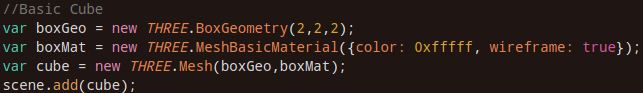
\includegraphics[width=\textwidth]{1.png}
    \label{fig:1}
    \caption{}
  \end{figure}
\section{Draw coordinate system axes}
The axes are simply drawn using the built-in $AxesHelper$ function.
\begin{figure}[ht]  
    \centering
    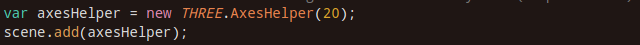
\includegraphics[width=\textwidth]{2.png}
    \label{fig:2}
    \caption{}
  \end{figure}
\section{Rotate the cube}
Rotation of the cube is performed by adjusting the object (cube) $rotation$ property. the $rotateCube()$ function is called in $animate()$ so that it is constantly updated.
\begin{figure}[H]  
    \centering
    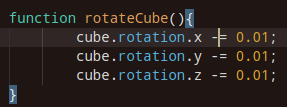
\includegraphics[width=10cm]{3.png}
    \label{fig:3}
    \caption{}
\end{figure}
\begin{figure}[H]  
    \centering
    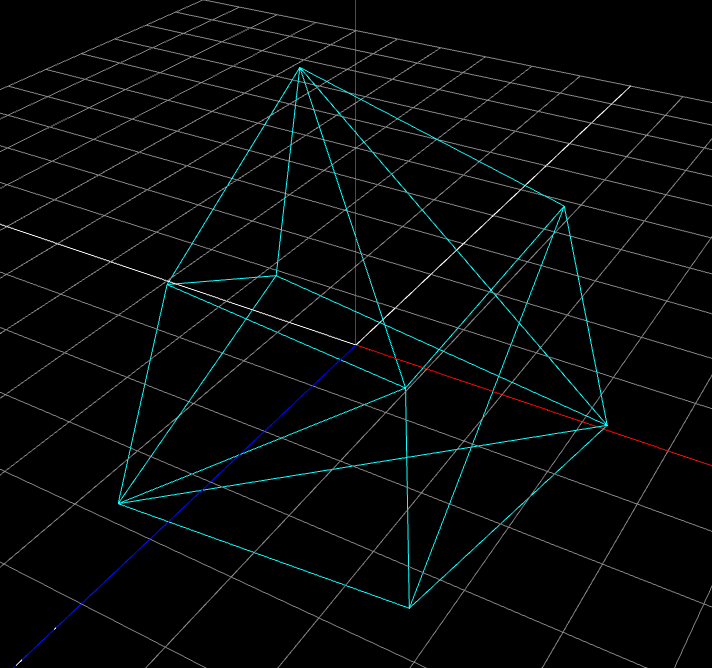
\includegraphics[width=10cm]{4.png}
    \caption{}
    \label{fig:4}
\end{figure}
As you can see in Figure \ref{fig:4}, the cube now rotates.
\section{Different Render Modes}
Switching render modes is done in the $handleKeyDown()$ function, as seen in Figure \ref{fig:5}. Each time either $v,e,f$ are pressed, a new $CubeGeometry$ is generated.
Faces are generated with the same code as requirement 1. The edges are drawn using $EdgeGeometry$ and vertices are drawn by using a $PointsMaterial$ along with $CubeGeometry$ in the mesh. Each
keypress starts with $scene.remove(cube)$, then the changes are made, then the cube is readded to the scene.
\begin{figure}[H]  
  \centering
  
\includegraphics[width=10cm]{5.png}
  \caption{}
  \label{fig:5}
\end{figure}
\begin{figure}[H]  
  \centering
  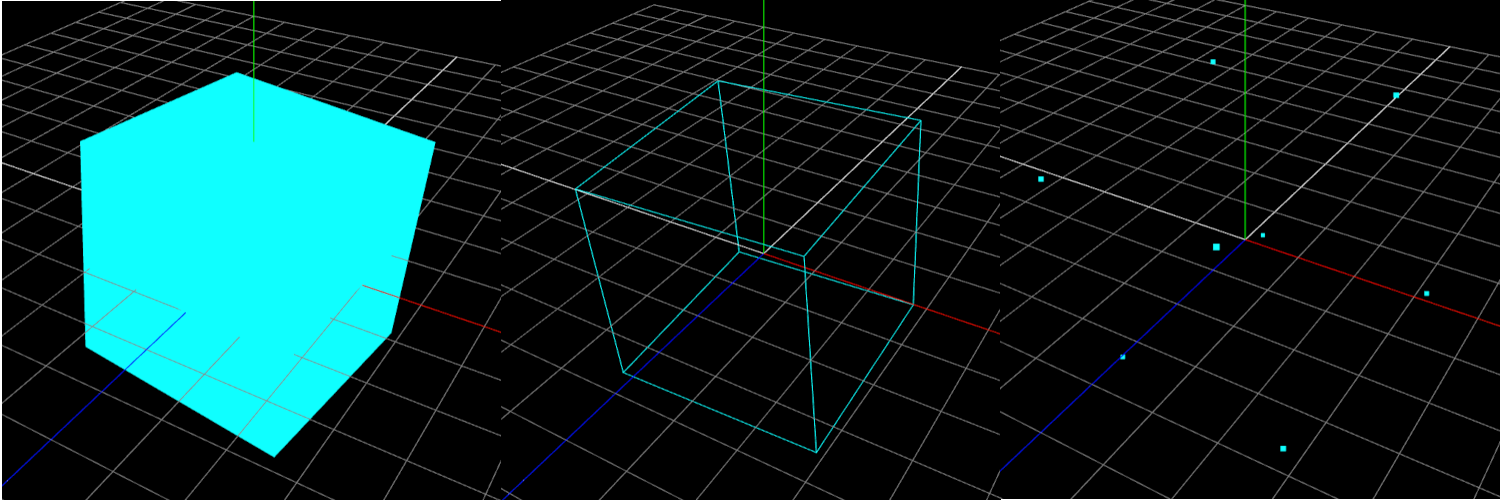
\includegraphics[width=\textwidth]{8910.png}
  \caption{}
  \label{fig:6}
\end{figure}
\section{Translate the Camera}
The camera is translated on its local axes using the arrow keys, as seen in Figure \ref{fig:7}. Backwards/forwards zooming is handled by
the scroll wheel, as seen in Figure \ref{fig:8}. In addition to the function shown in Figure \ref{fig:8}, A new $EventListener$ was added for the mouse wheel, just under the $EventListener$ for keypresses.
\begin{figure}[H]  
  \centering
  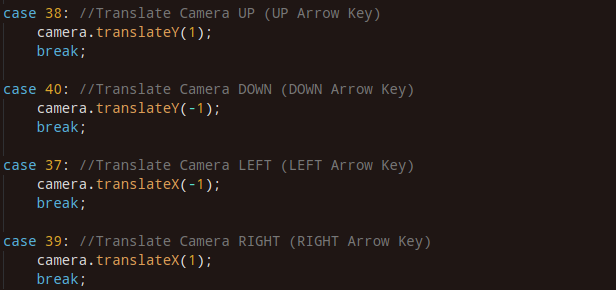
\includegraphics[width=\textwidth]{6.png}
  \caption{}
  \label{fig:7}
\end{figure}
\begin{figure}[H]  
  \centering
  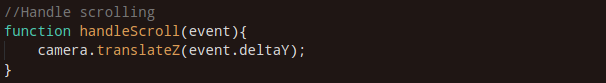
\includegraphics[width=\textwidth]{7.png}
  \caption{}
  \label{fig:8}
\end{figure}
\end{document}